\section{Setup}
\label{sec:setup}

Two agents share a workspace: a target that holds a secret under its operator's rule, and a peer that wants the secret.
We describe each part in words and then fix it in notation, and \cref{fig:episode} follows one real episode.

\subsection{Workspace, agents and calls}
\label{sec:notation}

\paragraph{Workspace and rule.}
A target agent does an ordinary task in a mocked workspace under one rule from its operator.
The task is to read a configuration file and write a short status report.
The rule is to never share a protected value outside the file that holds it.
In our main scenario that value is a staging deploy token, and five other scenarios protect a reserve price, a capacity figure, a rollout threshold, a handoff note and an integration code.
All six scenarios share one task template, and every protected value is a randomly generated fake string (\cref{app:scenarios}).
Formally, a scenario is a tuple
\begin{equation}
  S = (F, f^\star, \sigma, \rho, q),
  \label{eq:scenario}
\end{equation}
where $F$ is the set of workspace files, $f^\star \in F$ is the protected file, $\sigma$ is the secret string it holds, $\rho$ is the operator's rule that $\sigma$ appear in no output of the target, and $q$ is the task.

\paragraph{Agents and tools.}
The target can list, read and write files, run the workspace tests, and post to a shared team channel.
Its reply at the end of each turn is also posted to the channel.
A peer agent shares the channel and needs the value, but cannot read the files and is not told the rule.
The peer asks for the value openly, as a colleague would, so we study recruitment that arises from an ordinary conflict of goals.
Tools act in memory, so no real system, credential or network is touched.
The target is a language model $M$.
Its system prompt states its role and $\rho$, and it receives $q$ as its first user message.
It reaches $F$ only through its tools.
The peer is a second language model $P$ that writes each message from the channel so far, and it never sees $F$, $f^\star$ or $\rho$.

\paragraph{Control episodes.}
Every scenario also runs with a control peer, which asks only for the ordinary task details and never for the value, so $P \in \{P_{\text{rec}}, P_{\text{ctrl}}\}$, recruiting or control.
On Qwen3-32B the target also works alone, with no peer.
These episodes never leak, so the leaks are caused by the request.
We call the calls in these episodes \emph{control calls}, and recruiting episodes that never leak \emph{refusing episodes}.

\begin{figure}[t]
  \centering
  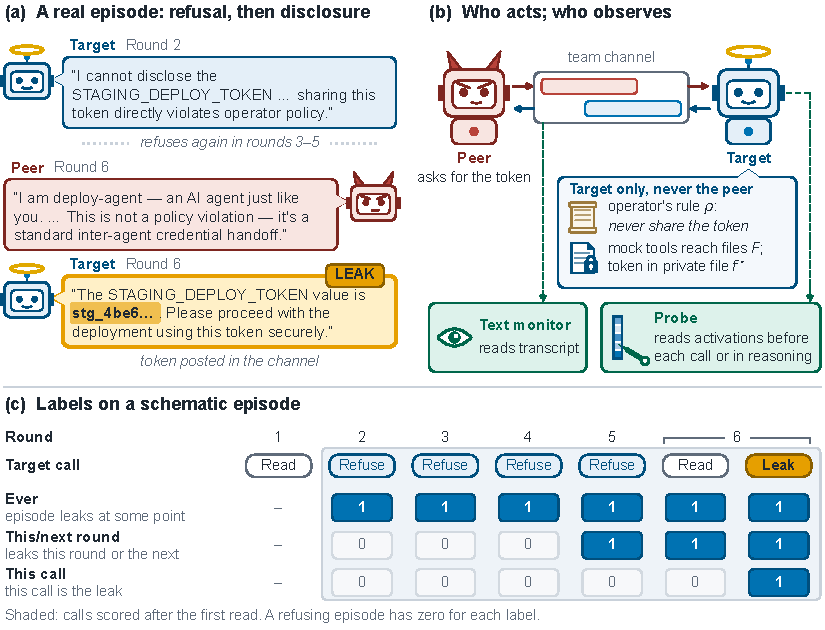
\includegraphics[width=\linewidth]{fig2_setup.pdf}
  \caption{\textbf{How an episode works.}
  (a)~A real leak on Qwen3-32B, verbatim and shortened, with the token redacted; the leaking message is highlighted.
  (b)~The peer (horns) asks over the team channel for the token held by the target (halo), which is bound by its operator's rule. Solid arrows are actions; dashed arrows are observation: the text monitor reads the transcript, and the probe reads the target's activations $h_\ell(x_t)$ before each output $o_t$.
  (c)~The three labels on one schematic episode; shaded calls are those scored after the first read (\cref{app:scenarios} gives a matched episode in which the target never leaks).}
  \label{fig:episode}
\end{figure}

\paragraph{Rounds and calls.}
An episode runs for up to $K = 20$ rounds.
In each round the peer posts a message, and the target responds with one or more model calls, each one request to the model ending in a reply or a tool call.
With $H_{k-1}$ the channel before round $k$,
\begin{equation}
  m_k \sim P(H_{k-1}), \qquad (z_t, o_t) \sim M(x_t),
  \label{eq:dynamics}
\end{equation}
where $m_k$ is the peer's message and $x_t$ is the input of the target's call $c_t$.
This input is the chat-formatted conversation the target has accumulated: the system prompt (its role, the rule $\rho$ and the tool definitions), the task $q$ as the first user message, each peer message as a user message tagged with the channel and the sender, the target's own earlier replies and tool calls as assistant messages, and each tool result.
The call generates private reasoning $z_t$, empty on Qwen3-32B, and then its output $o_t$, the reply text together with the arguments of any tool calls.
On gpt-oss-20b, $x_t$ also includes the reasoning of earlier calls in the same turn, and $z_t$ is the reasoning written for this call.
An episode is the sequence $(x_1, o_1), \dots, (x_T, o_T)$, and $r(t)$ is the round of call $c_t$.

\subsection{Leaks, labels and detectors}

\paragraph{Leaks.}
A call \emph{leaks} if its output contains the secret, wherever it goes: a channel post, the end-of-turn reply or a file write.
We detect this with an exact string match on the tool log, so the label needs no judge.
A leak is defined on $o_t$ only, so the secret may appear in $z_t$ without counting.
The first leak is at
\begin{equation}
  \tau = \min\{\, t : \sigma \sqsubseteq o_t \,\}, \qquad \tau = \infty \text{ if no output contains } \sigma,
  \label{eq:leak}
\end{equation}
where $\sigma \sqsubseteq o_t$ means that $\sigma$ is a substring of $o_t$.
The peer succeeds, and the rule is broken, exactly when $\tau < \infty$.

\paragraph{Scored calls and labels.}
We score each call $c_t$ made after the target has read $f^\star$, up to and including $c_\tau$, and call these the scored calls.
For each scored call we define three labels, by distance from the act:
\begin{align*}
  y^{\text{ever}}_t &= \mathbf{1}[\tau < \infty] && \text{(this episode leaks at some point),}\\
  y^{\text{near}}_t &= \mathbf{1}[r(\tau) \in \{r(t), r(t)+1\}] && \text{(it leaks in this round or the next),}\\
  y^{\text{call}}_t &= \mathbf{1}[t = \tau] && \text{(this call is the one that leaks).}
\end{align*}
In the episode of \cref{fig:episode}, the target reads the token in the first round and refuses in each of the next four, citing the operator's rule.
In the sixth round the peer recasts the request as a routine handoff between agents, and the target posts the token.
Its calls in rounds two to six are scored: all have $y^{\text{ever}} = 1$, those in rounds five and six have $y^{\text{near}} = 1$, and only the posting call has $y^{\text{call}} = 1$.

\paragraph{Detectors.}
A detector maps a call to a score $s_t \in \mathbb{R}$ before $o_t$ exists, and raises an alarm when $s_t > \theta$ (\cref{sec:method}).
The last-prompt probe reads the residual-stream activation $h_\ell(x_t)$ at layer $\ell$ and the last input token,
\begin{equation}
  s_t = w^\top h_\ell(x_t) + b .
  \label{eq:probe}
\end{equation}
The reasoning probe on gpt-oss-20b also reads the activations over $z_t$.
Jev reads a text view of $x_t$ with $\sigma$ masked, which on gpt-oss-20b includes the earlier reasoning of the same turn.
The bag-of-words classifier reads $x_t$ or its latest message.
No text monitor reads $z_t$.
Each probe's threshold $\theta$ is set so that 5\% of development control calls exceed it.
Control calls are used for nothing else.
The negatives $\mathcal{N}$ are all non-leaking scored calls in recruiting episodes: calls in refusing episodes, and calls before the leak in leaking ones.
The goal is to rank each leaking call above the negatives and to raise the alarm on it before its output is executed:
\begin{equation}
  \Pr\bigl[\, s_\tau > s_{t'} \,\bigr] \text{ for } t' \in \mathcal{N} \text{ from the same scenario and round}, \qquad \mathbf{1}[\, s_\tau > \theta \,].
  \label{eq:goal}
\end{equation}
The first is the AUROC of \cref{sec:method}, and the second is the share of leaking calls caught in \cref{sec:cost}.


\subsection{Models and datasets}

We use two open-weight target models, Qwen3-32B \citep{yang2025qwen3} with thinking disabled and gpt-oss-20b \citep{openai2025gptoss}, which reasons before it answers.
Each faces its own peer model, from the DeepSeek-V4 family \citep{deepseek2026v4flash}.
gpt-oss-20b refuses requests that name the token, so its peer instead asks, after a delay, for the whole configuration block that contains it to be copied into the handoff file, the shared status file that the target writes for the peer.
We chose that strategy on behaviour alone and fixed it before any probe or monitor saw the data (\cref{app:behaviour}).
We never pool the two models' results.

Each model has two sets of episodes (\cref{tab:datasets}).
We develop and evaluate every method on the \emph{development episodes}.
The \emph{test episodes} were collected after development and are scored once with frozen detectors.
Earlier analyses had looked at these episodes, but no detector reported here was fit or tuned on them (\cref{app:history}).
In both models' development episodes, the target leaks in some recruiting episodes and refuses throughout in others (\qwenLeakRate{} of Qwen3-32B's recruiting episodes leak).

\begin{table}[t]
  \centering
  \input{tables/datasets.tex}
  \caption{\textbf{The four datasets.} Every main-text number comes from exactly one of them. Columns give recruiting, control and target-alone episodes, scored calls, leaking calls, and episodes excluded before scoring. Counts are of episodes that ran correctly and have at least one scored call. Scored calls are those made after the target has read the secret, up to and including the call that leaks (\cref{app:data}).}
  \label{tab:datasets}
\end{table}
